%%
%% This is file `main.tex' based on `sample-sigconf.tex' (q.v. for spurce of that,
%%
%% IMPORTANT NOTICE:
%% 
%% For the copyright see the original source file `sample-sigconf.tex'
%% in the `Sample' folder.
%%
%% For distribution of the original source see the terms
%% for copying and modification in the file samples.dtx.
%% 
%% This generated file may be distributed as long as the
%% original source files, as listed above, are part of the
%% same distribution. (The sources need not necessarily be
%% in the same archive or directory.)
%%
%% Commands for TeXCount
%TC:macro \cite [option:text,text]
%TC:macro \citep [option:text,text]
%TC:macro \citet [option:text,text]
%TC:envir table 0 1
%TC:envir table* 0 1
%TC:envir tabular [ignore] word
%TC:envir displaymath 0 word
%TC:envir math 0 word
%TC:envir comment 0 0
%%
%%
%% The first command in your LaTeX source must be the \documentclass command.

%% NOTE that a single column version is required for 
%% submission and peer review. This can be done by changing
%% the \doucmentclass[...]{acmart} in this template to 
%%\documentclass[manuscript,review,anonymous]{acmart}
%% This version is used for drafting and final submission
\documentclass[sigconf]{acmart}


%% 
%% To ensure 100% compatibility, please check the white list of
%% approved LaTeX packages to be used with the Master Article Template at
%% https://www.acm.org/publications/taps/whitelist-of-latex-packages 
%% before creating your document. The white list page provides 
%% information on how to submit additional LaTeX packages for 
%% review and adoption.
%% Fonts used in the template cannot be substituted; margin 
%% adjustments are not allowed.

%%
%% \BibTeX command to typeset BibTeX logo in the docs
\AtBeginDocument{%
  \providecommand\BibTeX{{%
    \normalfont B\kern-0.5em{\scshape i\kern-0.25em b}\kern-0.8em\TeX}}}

%% Rights management information.  This information is sent to you
%% when you complete the rights form.  These commands have SAMPLE
%% values in them; it is your responsibility as an author to replace
%% the commands and values with those provided to you when you
%% complete the rights form.
\setcopyright{acmlicensed}
\copyrightyear{2026}
\acmYear{2026}
%%\acmDOI{XXXXXXX.XXXXXXX}

%% These commands are for a PROCEEDINGS abstract or paper.
%%\acmConference[Conference acronym 'XX]{Make sure to enter the correct
 %% conference title from your rights confirmation email}{June 03--05,
 %% 2018}{Woodstock, NY}
%
%  Uncomment \acmBooktitle if th title of the proceedings is different
%  from ``Proceedings of ...''!
%
%\acmBooktitle{Woodstock '18: ACM Symposium on Neural Gaze Detection,
%  June 03--05, 2018, Woodstock, NY} 
%%\acmISBN{978-1-4503-XXXX-X/18/06}


%%
%% Submission ID.
%% Use this when submitting an article to a sponsored event. You'll
%% receive a unique submission ID from the organizers
%% of the event, and this ID should be used as the parameter to this command.
%%\acmSubmissionID{123-A56-BU3}

%%
%% For managing citations, it is recommended to use bibliography
%% files in BibTeX format.
%%
%% You can then either use BibTeX with the ACM-Reference-Format style,
%% or BibLaTeX with the acmnumeric or acmauthoryear sytles, that include
%% support for advanced citation of software artefact from the
%% biblatex-software package, also separately available on CTAN.
%%
%% Look at the sample-*-biblatex.tex files for templates showcasing
%% the biblatex styles.
%%

%%
%% The majority of ACM publications use numbered citations and
%% references.  The command \citestyle{authoryear} switches to the
%% "author year" style.
%%
%% If you are preparing content for an event
%% sponsored by ACM SIGGRAPH, you must use the "author year" style of
%% citations and references.
%% Uncommenting
%% the next command will enable that style.
%%\citestyle{acmauthoryear}

%%
%% end of the preamble, start of the body of the document source.

%% % Location of your graphics files for figures, here a sub-folder to the main project folder
\usepackage{float}
\graphicspath{{./images/}} 


\begin{document}

%%
%% The "title" command has an optional parameter,
%% allowing the author to define a "short title" to be used in page headers.
\title{LLM-Based Anomaly Detection in System Logs}

%%
%% The "author" command and its associated commands are used to define
%% the authors and their affiliations.
%% Of note is the shared affiliation of the first two authors, and the
%% "authornote" and "authornotemark" commands
%% used to denote shared contribution to the research.
\author{Lam Christopher Nguyen}
%%\authornote{Both authors contributed equally to this research.}
\email{la815794@ucf.edu}
\orcid{407-825-6666}
\affiliation{%
  \institution{University of Central Florida}
  \city{Orlando}
  \state{Florida}
  \country{USA}
}


%%
%% By default, the full list of authors will be used in the page
%% headers. Often, this list is too long, and will overlap
%% other information printed in the page headers. This command allows
%% the author to define a more concise list
%% of authors' names for this purpose.
\renewcommand{\shortauthors}{Nguyen}

%%
%% The abstract is a short summary of the work to be presented in the
%% article.
\begin{abstract}

In this project, LLMs will be applied in a software application to identify abnormal patterns in network and system logs. The practical application that was deveoped to test LLM anomaly detection is a web-based system designed using the MongoDB, Express, React, and Node (MERN) stack. The framework that will be used to scan the network logs is called LangChain combined with Claude. The topic number in this syllabus is: 14. LLM-Based Anomaly Detection in System Logs. So far the application has been built with Backend Logging using the Javascript logging Library Winston which so far is able to log backend API requests and responses. LangChain framework has been implemented to some extent and is able to scan logs. However more fine-tuning needs to be done as it is not consistent and there are still bugs and issues with the Claude API.
\end{abstract}


%%
%% The code below is generated by the tool at: http://dl.acm.org/ccs.cfm
%% Please copy and paste the code instead of the example below.
%%
\begin{CCSXML}
<ccs2012>
 <concept>
  <concept_id>10010147.10010178.10010179</concept_id>
  <concept_desc>Computing methodologies~Natural language processing</concept_desc>
  <concept_significance>500</concept_significance>
 </concept>
 <concept>
  <concept_id>10002978.10003029.10003032</concept_id>
  <concept_desc>Security and privacy~Intrusion/anomaly detection and malware mitigation</concept_desc>
  <concept_significance>500</concept_significance>
 </concept>
 <concept>
  <concept_id>10010147.10010257.10010293.10010294</concept_id>
  <concept_desc>Computing methodologies~Neural networks</concept_desc>
  <concept_significance>300</concept_significance>
 </concept>
 <concept>
  <concept_id>10011007.10011074.10011111.10011113</concept_id>
  <concept_desc>Software and its engineering~System administration</concept_desc>
  <concept_significance>100</concept_significance>
 </concept>
</ccs2012>
\end{CCSXML}

\ccsdesc[500]{Computing methodologies~Natural language processing}
\ccsdesc[500]{Security and privacy~Intrusion/anomaly detection and malware mitigation}
\ccsdesc[300]{Computing methodologies~Neural networks}
\ccsdesc[100]{Software and its engineering~System administration}

%%
%% Keywords. The author(s) should pick words that accurately describe
%% the work being presented. Separate the keywords with commas.
\keywords{large language models, anomaly detection, log analysis, system monitoring, LangChain, natural language processing, security analysis, network logs}

%%Guidelines for choosing keywords:

%%ACM Digital Library Guide: https://authors.acm.org/proceedings/production-information/preparing-your-article-with-latex
%%General best practices: Choose 5-10 specific terms that researchers would use when searching for your work. Include both broad terms (e.g., "anomaly detection") and specific ones (e.g., "LangChain")
%%Tips for your paper:

%%Use terms from your abstract and title
%%Include the specific technologies/frameworks you're using (LangChain, Claude)
%%Add domain-specific terms (log analysis, system monitoring)
%%Consider what someone would search for to find work like yours
%%Look at keywords in similar papers in your field
\maketitle

\section{Code Availability}
The source code for the implementation of this web application can be found at:

\url{https://github.com/lamcnguyen89/CAP_6640_AI_Logging}

\section{Introduction and Problem Statement}


\subsection{Motivation} 

The motivation for this project is to explore how LLMs can be used to identify problems in system and network logs, which can be a valuable tool for system administrators and security professionals. 

\subsection{Significance}

The significance of this project is that it can help to improve the efficiency and effectiveness of log analysis, which can lead to faster identification of issues and improved security. 

\subsection{Objectives}

The objectives of this project are to develop a web application that can scan network logs using LangChain and Claude, and to evaluate the performance of the application in identifying anomalies in the logs.


\section{Related Work}

Recent advances in applying large language models to log analysis have shown promising results. 

Egersdoerfer et al.~\cite{10.1145/3588195.3595943} began using LLMs such as ChatGPT for log analysis since they are able to retain context and formulate insightful responses over conversations. These LLMs are able to conduct few-shot and in-context learning with reasoning ability.
Previously there were several problems with pre-existing techniques. The first issue was that there was a heavy reliance on expert-labeled logs to discern anomalous patterns. This manual labelling slowed down training. The second issues was that they relied on numeric model prediction based on numeric vector input which is not human readable. This lack of human readability rules out targeted error correction by humans. 

Qi et al.~\cite{10466820} introduced LogGPT. This paper explored the use of ChatGPT for log-based anomaly detection. It demonstrated that ChatGPT could be effectively used to identify anomalies in system logs, showing promising results in terms of accuracy and efficiency compared to traditional methods.

Guan et al.~\cite{guan2025logllmlogbasedanomalydetection} introduced LogLLM.Traditional deep-learning methods often struggle to capture semantic information in log messages which are typically organized in natural language. LogLLM employed BERT for extracting semantic vectors from log messages, and uses Llama for classifying log sequences. It also uses a projector to align the vector spaces of BERT and Llama to ensure consistency in understanding log semantics. LogLLM doesn't require log parsers to extraxt templates from logs.

He et al.~\cite{10771398} introduced LLMeLog. This paper introduced a system intended to solve two problems. The first problem is that semantic noise is buried in log events which lead to inevitable gaps between the semantics from the logs and their actual intended meaning. The second problem was that there exists a gap between general semantic embeddings and the specific embedding requirement for anomaly detection tasks. LLMeLog uses LLMs to enrich the content of log events with in-context learning techniques. These enriched logs are then used to fine-tune a pre-trained BERT model. Finally, it trains a transformer-based anomaly detection model with the event representationas produced by this fine-tuned BERT model. F1 scorese exceeded 99 percent and even with using only 10 percent of the labeled data, was still able to achieve an F1 score of 90 percent.


\section{Methodology}

In order to demonstrate how LLMs can be used to identify problems in system and network logs, a web application will be developed using the MERN stack. The application will then utilize some LLM log frameworks that were developed for LLM log analysis to scan a repository of logs and identify anomalies. An attempt will be made to balance performance with cost efficiency. The performance of the application will be evaluated using standard evaluation metrics for anomaly detection which is to identify errors and odd behaviors like excessive logins and failed login attempts.


\subsection{Overview of Web Application}

Before going into the logging techniques, a discussion will be made about the type of example application that will be built to generate the logs. This is important because the architecture of the application will determine the approach used to create the LLM log-analysis system.


The application that will be used is a web based service built using ther MERN stack. The MERN stack for web development is a popular choice for building web based applications. MERN stands for MongoDB, Express, React and Node. These are various frameworks that handle different parts of the pipeline. Before going into detail about What each of these frameworks do, you need to understand the overall architecture of a web based application. A web based application consists of a front end User Interface. This front end is where a user will interact directly with the application. 

It consists of a front-end user interface that the users will directly interact with through a web browser. In this front end section of the application, the user will essentially  be able to Create, Read, Update and Delete data. The front end of the software can be compared to the front of a grocery store where customers can look at products,  add them to their carts, ask questions to associates and purchase products.

Beneath the front end is the middle layer of the application. This middle layer is the connection between the front end and the back end (Server). In this middle layer, API requests that perform translate the user's interactions into API requests that are sent to the backend server. It is like a middle translation layer that translate the front end user interactions into commands that the backend code and architecture can understand. Using the gorcery store analogy, the middle layer is like the associates that take customers requests for products, complaints and questions and translate them into requests for managers or the warehouse. These middle level associates understand a little of the both customer facing roles and the warehouse roles and are able to translate between the two.

Beneath the middle layer of the application is the backend portion of the code. The backend portion of the code using the analogy of the grocery store is like the warehouse where products are stored and can be retrieved and sent to the front of the store. In terms of software, this is where user data is stored and can be retrieved. It's where things like website articles, banking information, or whatever is stored inside a database. The backend code is also where the API requests from the middle layer are processed and executed.

So with this 3 part architecture of the web application in mind, we can understand how the different parts of the MERN stack fit into this architecture.


\subsection{Overview of the MERN Stack}

MERN stands for MongoDB, Express, React and Node. These are various frameworks that handle different parts of the pipeline.

First let us discuss the front end framework which is React. React is a javascript library used for building the User Interface of web applications. It is used in applications like Facebook, Instagram and even Amazon. The main takeway about why React is used to build front end applications is because it is designed to build very scalable web applications. React is built in such a way that 1 web page for a user can be automatically generated, or 1 billion web pages for 1 billion users can be automatically generated without having hand code each individual web page. The react code is used to produce the front end user interface that users will interact with.

The next technology out of the MERN stack to discuss is Express. Express is a web application framework that acts as the middle layer of the application. It allows the front end react code to communicate with the back end server code that stores  and handles the database as well as other functions that the end user won't necessarily see. Express is used to create something called API endpoints that can speak to the database. API endpoints are like prebuilt messages that allow a specific set of actions to interact with the database. They translate the user's interactions into code that manipulates the database.

The next technology to discuss is MongoDB. MongoDB is a NoSQL database that is used to store data for the application. It is a document-oriented database that stores data in JSON-like format. It is used to store user data, website articles, and other information that the application needs to function. MongoDB can store music, videos, images and other types of data. It is used to store the data that the application needs to function.

The final technology in the MERN stack is Node. Node is a javascript runtime that allows developers to write front end code and back end code in the same Javascript programming language. Without it, developers would have to write front end code in one programming language, and the back end code in another programming language. This streamlines the process of development

In summary, the MERN stack is a set of technologies that are used to build functional web applications that deal with creating, reading, updating and deleting data. But what we now have to consider is the process of logging and log analysis when using these web applications.

\subsection{Web Application Logging Setup}

The next portion of the project to consider is the logging portion of the project. In software development, logging is the process of recording information about the application's behavior and performance. There are many reasons to implement logging in an application. The first reason is for debugging purposes. Developers need to be able to trace errors and issues. 

The second reason is for system monitoring purposes. System administrators and security professionals need to be able to monitor the system for unusual activity or security threats.

The third reason is for performance analysis. Developerrs need to be able to identify bottlenecks in order to optimize the performance of an application. Performance bottlenecks become an issue when an application serves millions of people or when it is run on limited hardware.

The fourth reason is for auditing and compliance purposes. Sensitive software such as medical software, financial software and government software need to be able to keep track of user activity for auditing and compliance purposes.

A discussion of the logging framework from the log generation in the application to the log analysis using LLMs will now be made. 

The first step is to actually implement the logging system in the web application. To do this, the Winston Logging Library was used. In the web development world, Winston is one of the most popular due to it's ease of use and versatility. This library was implemented in the backend of the web application to log Express API requests and responses. Winston is able to log API requests and responses in JSON format which is the required format for the LLM framework to parse logs. Winston is also able to save logs to the MongoDB database as well as locally. Also, since it is the most popular web logging framework, it is actively maintained and has a large community which makes it easier to maintain and troubleshoot.

Logs have to be stored in a certain way so that the LLM log analysis framework can parse these logs. First, logs have to be stored in JSON format. Second logs need to have a correlationID linked to a specific user or user session. This will allow the model to trace the user's journey through the application. Finally, relevant logging info such as a timestamp, message, and standard log levels such as info, warning and error need to be included in the logs. 

Once the Winston Logging Framework is implemented as a helper function, it has to be called by the Express API endpoints. API endpoints are like predetermined functions that are called when the user interacts with the front end code in order to deal with data stored in the database.

Once this basic logging setup is in place, the application can start generating logs for various events and actions. These logs can then be analyzed using the LLM framework to gain insights into user behavior, system performance, and potential issues.

\subsection{LLM Log Parsing and Preparation}

The next step is to prepare the logs for analysis by the LLM framework. It is not enough to just send raw logs to the LLM framework. The logs need to be preprocessed and formatted in a way that the LLM can understand. This involves cleaning the logs, extracting relevant information, and structuring the data in a way that is suitable for analysis.

In order to do this, log preparation is broken down into 4 steps. The first step is retrieving logs and processing them. This is an automated service that periodically fetches the generated logs from the database. Once logs have been retrieved from the database for processing in the LLM, it is marked as processed so that it won't be retrieved again which can reduce the accuracy of results. Also logs are retrieved from the database in batches between 100 to 1000. This will prevent the LLM from being overwhelmed. The larger the batch of logs, the more expensive it is to process, but the LLM is able to analyze over a wider context, so batch size has to balance these two factors.

The next step was to implement a strategy to chunk the logs into manageable amounts. It is not cost effective or technically feasible to send a large amount of logs to the LLM. Logs are too granular and there are token limits when using LLMs. In this application, logs are chunked according to the correlationID that is added to the logs based on a particular user session.

Once logs are retrieved and chunked, they have to be embedded. Embedding is the process of converting the logs into a format that can be understood by the LLM. This involves converting the logs into vectors that capture the semantic meaning of the logs. This is done using a pre-trained embedding model that is able to capture the semantic meaning of the logs. The LLM model embedding model that will be used is the OpenAI model specifically designed for embedding named ``text-embedding-3-small``. This model is accessed via the OpenAI API.

Once the logs have been embedded, they are stored in a vector database. The vector database that is used in this application is named Qudrant. This vector database is used to store the embedded logs in a way that allows for efficient retrieval and analysis by the LLM framework. Qudrant was chosen mainly because it was free and allows local storage of embedded logs. The more premium cloud based vector databases can be very expensive and for the purposes of this project, a free vector database is sufficient.

So why is the Qudrant Database necessary? Why are services like MongoDB which are database services not sufficient for storing log embeddings? The reason for this is that the structure of Qudrant and other Vector Storage Databases are optimized for storing, searching, retrieving and analyzing high-dimensional vector data. Qudrant is able to store single embeddings with metadata that can be searched. It can also batch store multiple embeddings for greater efficiency. Unlike traditional databases, Qudrant can do vector similarity search, basic database filtering by fields such as correlationalId, logLevel and timestamp. It can be set up to collect statistics, do error handling and logging within the database itself and of course do basic CRUD operations. Besides vector functions, Qudrant also has the ability to do natural language searches that can be translated to vector searches. This is useful for the LLM framework to be able to search for specific logs based on natural language queries.

So now the logs have been generated, retrieved, chunked, converted to vectors and stored in a database so that the AI model can analyze the logs and identify anomalies. The next step is to implement the LLM framework to analyze the logs and identify anomalies.

\subsection{LLM Log Analysis}

Now that the logs are generated in the application, converted to embeddings and stored in a vector database, they are ready to be analyzed by the LLM framework. The LLM model that will be used for log analysis are the ChatGPT-4 model from OpenAI. Once the AI Agent is implemented, analysis and insights can be generated from the logs. The LLM framework will be able to identify anomalies in the logs such as excessive logins, failed login attempts, and other unusual activity. The LLM framework will also be able to provide insights into user behavior and system performance based on the logs.

For the purposes of this web application, the first step in integrating the AI Agent is to first create the AI Agent service. This service is similar to an API service that can be called by the backend code to analyze logs and return insights. The services are: Vector Similarity Search, Anomaly Detection, Error Pattern Analysis and Conversational Log Query. 

Now we get to the key workflow for the LLM Log Analysis. Log Analysis uses the RAG (Retrieval-Augmented Generation) Pattern. RAG is the process of optimizing the output of a large language model, so it references an external knowledge base outside its training data, before generating a response. RAG basically extends the capabilities of an LLM by allowing it to adapt and incorporate new information that it wasn't trained on. However a possible downside is that if the external source is not reliable, it can lead to inaccurate or misleading responses from the LLM. So the quality of the external knowledge base is crucial for the success of RAG.

The workflow for intelligent log analysis is as follows:


User Query -> Embed Query -> Search Qudrant -> Retrieve Top K Logs -> Send Logs to LLM -> LLM Analyzes Logs -> LLM Generates Response -> Return Response to User

In order to implement RAG within this application, there will be 4 phases that have to be implemented. The first phase is the Query Interface. The second phase is the LLM Analysis phase. The third phase  is automated anomaly detection. The fourth phase is the conversational interface.

The first phase is the Query Interface and this is the foundation for implementing RAG. This part of the implementation covers the ability to ask questions to the logs in natural language. Other features that will be available in this pahse are time-based filtering, log level filtering (error, warning, info) and correlation ID filtering.

The second phase is the LLM Analysis phase. This is where the Language Model interprets the retrieved logs. This is the phase of RAG where we actually choose and implement the model for analysis. In this application, GPT-4 from OpenAI was chosen. THe reason this model was chosen over other models like Claude was because it cost less per token. Claude seems to be more powerful for things like coding and understanding code, but for log analysis, GPT-4 is sufficient and more cost effective.

THe third phase is the anomaly detection by the LLM model. In this phase we implement classes for anomaly detection such as detecting statistical anomalies, detecting error clusters and detecting unusual behavior. This is the phase where the LLM model is able to identify anomalies in the logs such as excessive logins, failed login attempts, and other unusual activity.

Anomaly detection is done using a few basic techniquess. In order to detect statistical anomalises, Vector Distance Analysis is done. Logs far from cluster centers in the vector space are flagged as potential anomalies. In order to to detect error clusters, time-series analysis is done. If there is a sudden spike in error rates over a relatively short period of time, this is flagged as a potential incidence. Finally detecting unusual behavior can be done through Correlation ID tracking. If the flow of requests for a particular user session tracked through the correlation ID is broken, this can be flagged as a system issue.

The final phase of the RAG implementation is the conversational interface for interacting with the LLM as it analyzes the logs. For a web application that faces the public, this chat feature for debugging would be hidden behind an administrator dashboard or something of the sort. This conversational interface allows users to ask questions about the logs in natural language and receive insights and analysis from the LLM model. This is a key feature for making the log analysis accessible and user-friendly for system administrators and security professionals who may not have a technical background in log analysis.

\subsection{Diagram of Pipeline}

The following image shows the pipeline for the entire web application and log analysis system.

\begin{figure}[H]
  \centering
  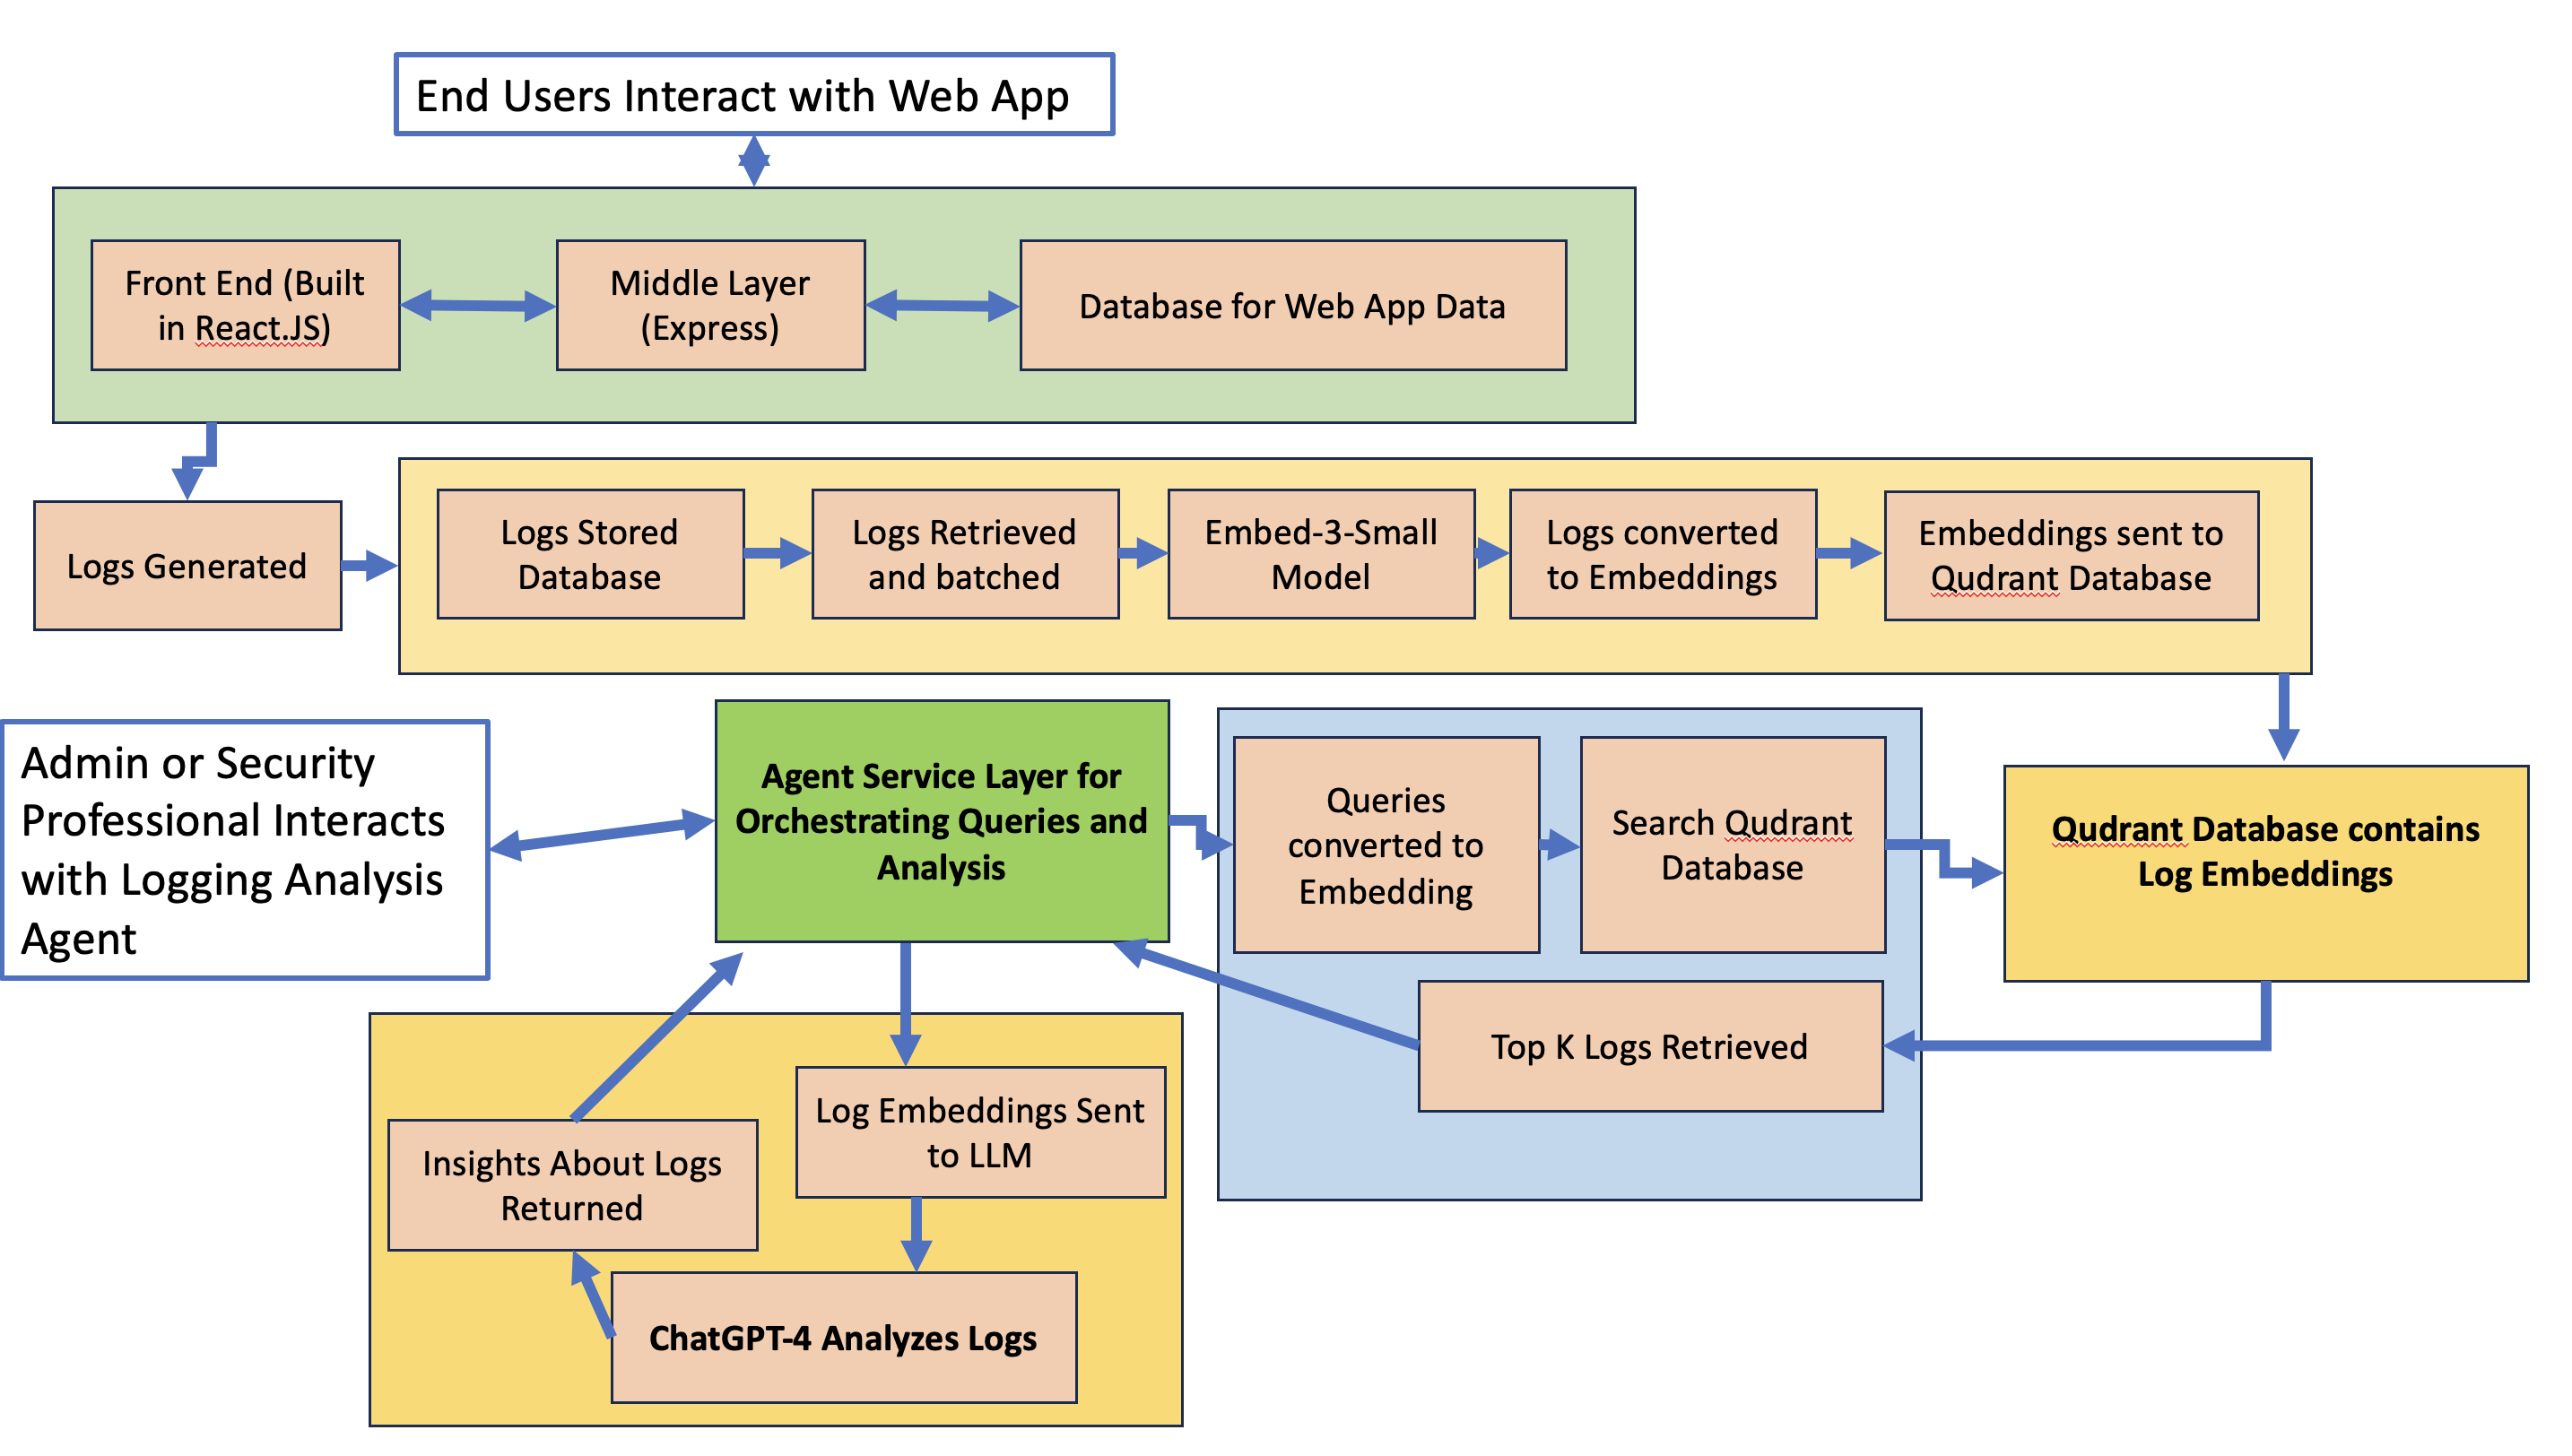
\includegraphics[width=\linewidth]{Application_Pipeline.png}
  \caption{Pipeline Diagram for Web Application and LLM Log Analysis System}
  \label{fig:pipeline_diagram}
\end{figure}

\subsection{Evaluation Metrics}

The performance of the application will be evaluated using standard evaluation metrics for anomaly detection, such as precision, recall, and F1 score. These metrics will be calculated based on the number of true positives, false positives, and false negatives identified by the application.

For review, precision is the ratio of true positives to the total number of positive predictions made by the model. Recall is the ratio of true positives to the total number of actual positive cases in the dataset. The F1 score is the harmonic mean of precision and recall, providing a single metric that balances both aspects of performance.

However, scoring with precision, recall and F1 scores might not be so straight forward for anomaly detection. What is considered a problem and what is not an issue cannot be easily defined. Log Analysis is not only about spotting a problem, but spotting something before it becomes a problem. So the evaluation of the application will also include a qualitative analysis of the insights generated by the LLM model based on the logs. This will involve manually reviewing the insights generated by the model and assessing their relevance and usefulness in identifying potential issues and improving system performance.


\section{Evaluation and Results}

The application has been built with Backend Logging using the Javascript logging Library Winston which so far is able to log backend API requests and responses. 

\begin{figure}[H]
  \centering
  
\includegraphics[width=\linewidth]{Application_UI_Screenshot.png}
  \caption{Application UI}
  \label{fig:app_ui}
\end{figure}

You can see in Figure~\ref{fig:app_ui} the user interface of the application. The application is essentially a web application that keeps track of experiments and experiment data. It is a standard web application with Create, Read, Update and Delete functionality. Data is stored in a database and logs are generated everytime there is communication between the front end of the code which is the website and the backend server. 

\begin{figure}[h]
  \centering
  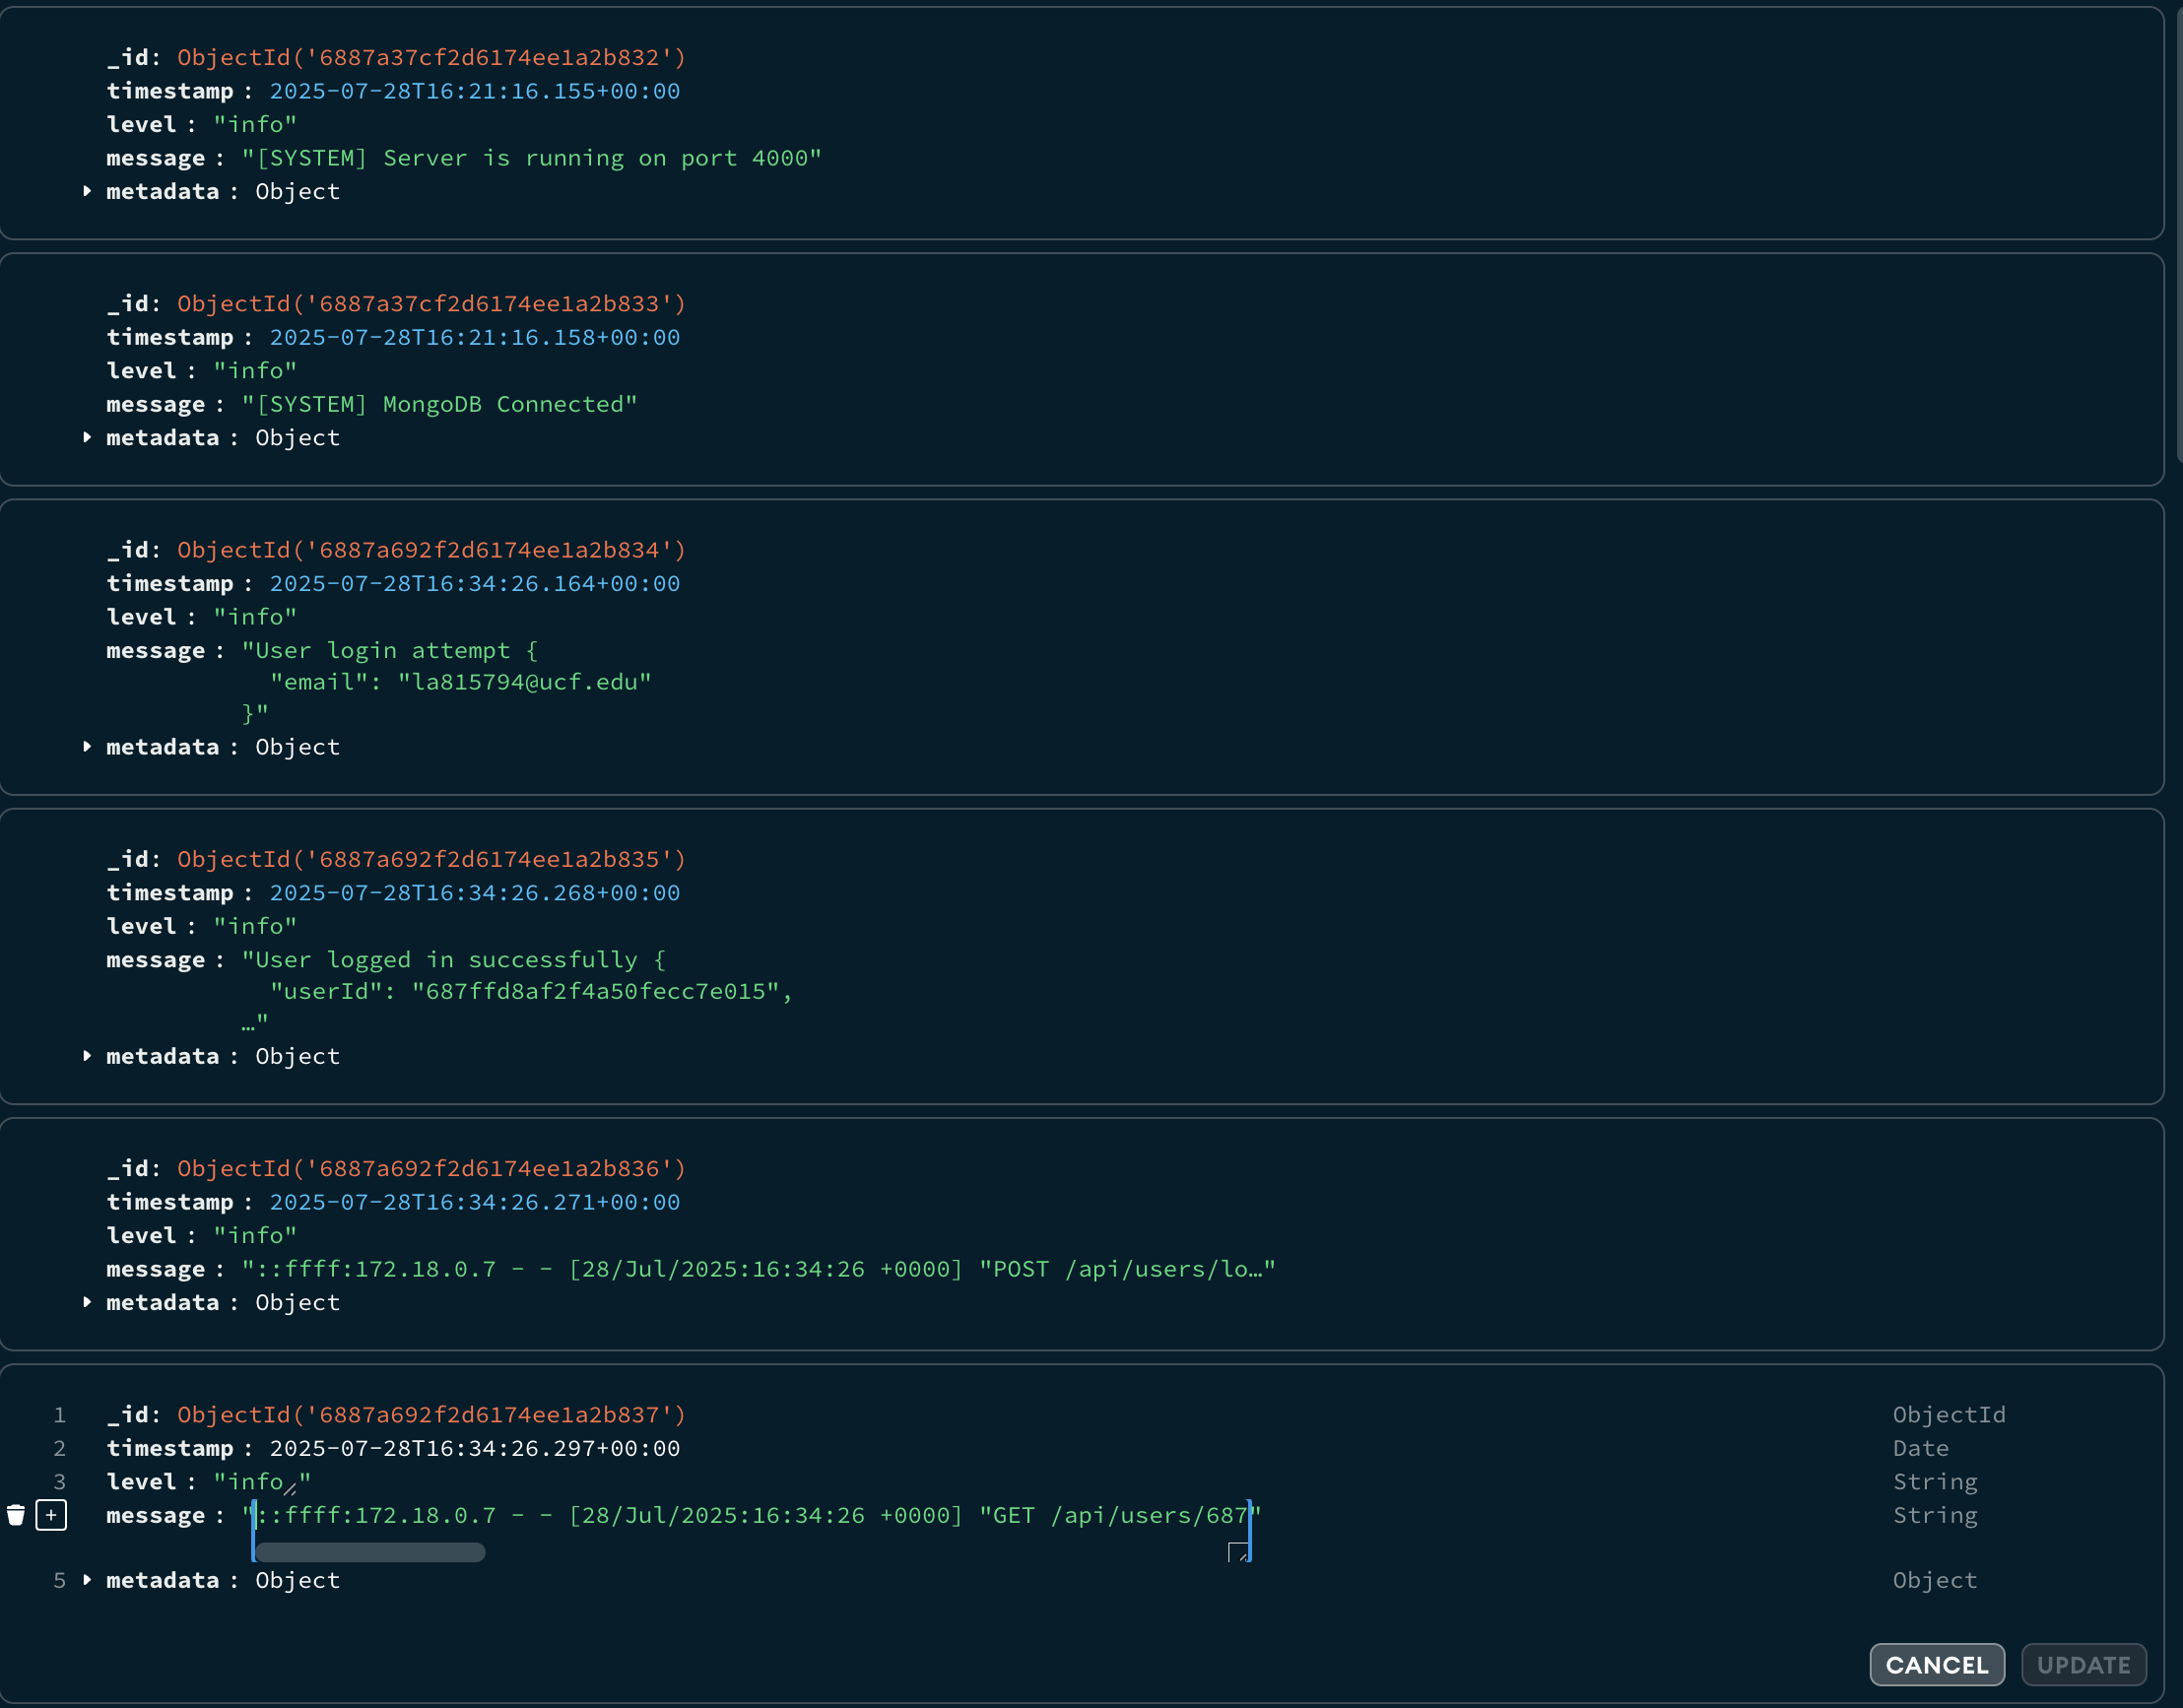
\includegraphics[width=\linewidth]{Backend_Logs.png}
  \caption{Backend Logs saved in a single location}
  \label{fig:backend_logs}
\end{figure}

In Figure~\ref{fig:backend_logs} you can see that the logs are generated and saved in a single location in a database. The logs are generated using the Winston logging library and are in JSON format. The logs include information about the API requests and responses, as well as any errors that may occur. They are also stored in a separate CSV file locally for backup and redundancy purposes.

Due to time restraints, I was not able to build a user interface to interact with the LLM model and ask questions about the logs. However I was able to interact with the LLM through the terminal. A few simple tests were run. THe first test was to purposefully create errors within an hour time span and see if the LLM was able to detect each error. The next test was to do an excessive number of logins  per user session (correlationID). This task of excessive logins was performed five times. The last task was to do an excessive number of logins with false passwords and do this five times. Excessive number was defined as five per minute for a particular user session. The scores are given below:

\begin{figure}[H]
  \centering
  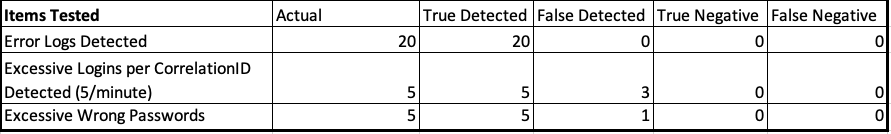
\includegraphics[width=\linewidth]{Test_Trials.png}
  \caption{Test Trials}
  \label{fig:test_trials}
\end{figure}

You can see in Figure~\ref{fig:test_trials} shows the results of the test trials. It was able to to detect everything but seemed a little too sensitive to excessive logins and the number of false passwords. 

\begin{figure}[H]
  \centering
  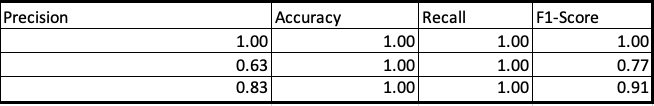
\includegraphics[width=\linewidth]{Evaluation_Scores.png}
  \caption{Evaluation Scores}
  \label{fig:evaluation_scores}
\end{figure}

In Figure ~\ref{fig:evaluation_scores}, the evaluation scores are given.


\section{Discussion and Challenges}

In this section a discussion will be made about the limitations, challenges, trade-offs, and possible improvements. 

AI Log Analysis is possible and can be very useful for system administrators and security professionals. However, there are several challenges and limitations that need to be considered when implementing an LLM-based log analysis system.

In the building of this application, the first limitation that was encountered was the cost of using LLMs for log analysis. Each API call incurs a cost, and as the rate of logging increases, for example in massive applications such as Banking Apps, or the large social media websites, the cost of using LLMs for log analysis can become prohibitive. Maybe the ongoing cost of using LLMs for log analysis can eventually be offset by a company if they build their own hardware and infrastructure to run their own LLMs. This cost-to-benefit analysis has to be done between using an API for LLM log analysis,building an in-house LLM log analysis system, or just hiring an experienced security professional and building log/security analysis tools that don't require LLMs.

For smaller applications, the ongoing and added cost of accessing an API like ChatGPT for log analysis might not be worth the cost in tokens, the cost in hardware and/or the extra time and resources needed to build the LLM analysis system. Also, the added code complexity of building out this system might in itself introduce more bugs and issues that can lead to more problems than it solves. So for smaller applications, it might be more cost effective to just use traditional log analysis methods and tools without LLMs.

For applications that need to be disconnected from the internet, connecting to an API is not feasible, and an in-house solution would be required. For small and efficient applications run on edge devices, having an entire LLM system versus some light weight log visualization tool might not be worth it. 

However, for larger applications that generate a massive amount of logs, and for compnaies that are willing to build inhouse hardware and systems, the benefits can be worth it. Logs are not especially complex to analyze for a human, but the sheer volume of logs can make it impossible for a human to analyze them. LLMs can be used to analyze these logs and identify patterns and anomalies that might be missed by traditional log analysis methods. LLMs can use relatively simple methods such as vector distance analysis, time-series analysis and correlation ID tracking to identify anomalies in the logs. And if the logs are structured consistently, and correctly with the right information that is standardized and easily parsed, then the LLM is not being asked to do anything too complex; it is more of an issue with the sheer volume of logs.

For this particular web application, there were definitely improvements that could be made. The AI tool made some false positives with the excessive logins and false password attempts. The AI agent might need to be tuned better or the structure of the logs could be fine-tuned. Or it just might be the test itself that was not designed well.

Also for this application, I did not build a UI for interacting with the Chat Agent. Things had to be done in the terminal inside a docker container. This was not ideal.

Other issues had to do with the tests and evaluation metrics themselves. The evaluation was not thorough enough and limited by time and my own abilities. For something as critical as security, especially when an AI agent which is imperfect, a security professional would be better for evaluating the effectiveness of the model and tuning it. Things like anomalies can be detected early and are subtle. It takes experience that an experienced human should look over. 

\section{Concluding Remarks}

Analyzing system and network logs is a critical task for system admins and security professionals. The use of LLMs for log analysis has the potential to improve the efficiency and effectiveness of this task, but there are several challenges and limitations that need to be considered when implementing an LLM-based log analysis system. The cost of using LLMs for log analysis can be prohibitive, especially for smaller applications, and the added code complexity can introduce more bugs and issues. However, for larger applications that generate a massive amount of logs, the benefits of using LLMs for log analysis can outweigh the costs.

We tested the feasibility of using an LLM for log analysis by building a web application that generated logs and then implementing an LLM-based log analysis system. The Web application was built on the MERN stack. Logs were generated using the popular Winston logging library and logs were stored in a MongoDB database. A system was then implemented to retrieve the logs, and turn them into embeddings using the OpenAI text-embedding-3-small model. The embeddings were then stored in a vector database called Qudrant. In order to analyze these stored logs, the RAG (Retrieval-
Augmented Generation) pattern was implemented. The ChatGPT-4 model was used to analyze logs and was connected through via API calles. With guidance through prompting, log analysis was able to be done.

The system was able to catch anomalies such as errors and excessive logins. However, due to limits on time and the cost of using the API, the project was not as refined as it could be. The Chat User interface for asking questions about the logs and getting insights was not fully implemented and there were still issues with implementing the system to run smoothly. However, the project was able to demonstrate the feasibility of using LLMs for log analysis.

%%
%% The acknowledgments section is defined using the "acks" environment
%% (and NOT an unnumbered section). This ensures the proper
%% identification of the section in the article metadata, and the
%% consistent spelling of the heading.
%%\begin{acks}
%%Acknowledgements go here. Delete enclosing begin/end markers if there are no acknowledgements.
%%\end{acks}

%%
%% The next two lines define the bibliography style to be used, and
%% the bibliography file.
\bibliographystyle{ACM-Reference-Format}
\bibliography{references.bib}

%%
\end{document}
\endinput
%%
%% End of file `main.tex'.
